\section{Matter (\textit{Rūpa})}

Welcome to the fifth talk of this Practical Abhidhamma Course.\footnote{More details in Chapter 6 of “A Comprehensive Manual of Abhidhamma” and “The Buddhist Teaching on Physical Phenomena (see footnote 2).} This talk will describe Matter, the third of the four Ultimate Realities (\textit{citta}, \textit{cetasika}, \textit{rūpa} and \textit{Nibbāna}). You should have the \textit{Satipaṭṭhāna} Sutta printout, Handout 2 and Handout 5 in front of you.

Handout 5 has two sections. The left side of Handout 5 is a glossary like Handout 3, listing and defining each \textit{rūpa}. The right side of Handout 5 is a chart listing groups of \textit{rūpas} across the top, then showing which \textit{rūpas} are included in each group. \textit{Rūpas} never arise in isolation; they are always part of a group. As shown in Handout 5, groups of \textit{rūpas} can arise from different causes; some groups are temperature-born, some are kamma-born, some are mind-born and some are nutriment-born.

The Pāḷi word “\textit{rūpa}” is usually translated as matter, but as we will see, \textit{rūpa} includes more than what is conventionally called matter. \textit{Rūpa} includes all non-mental phenomena and so in this talk, I will use the Pāḷi word “\textit{rūpa}” rather than the English word “matter.” During a Dhamma talk on \textit{rūpa}, I remember the monk saying, “What is matter? Never mind. What is mind? Doesn’t matter.” Actually, mind is very important because spiritual development is the training of the mind. Matter is important because it is an object of the mind, plays a role in bringing sense objects into the mind, and the physical body is made up of \textit{rūpas}.

Consciousness and Mental Factors experience objects, whereas \textit{rūpa} does not know anything. Consciousness, Mental Factors and \textit{rūpas} are impermanent; they arise for a moment and then pass away. It may seem that \textit{rūpas} such as smoothness or temperature can last, but the smoothness or temperature that is experienced now is different from the smoothness or temperature that arose a moment ago.

When analysing a cup of coffee, a scientist might break it into solid (the cup), liquid (the coffee) and gas (the aroma). According to the Abhidhamma, a cup of coffee consists of \textit{rūpas} such as \textbf{Hardness}, \textbf{Roughness}, \textbf{Heaviness}, \textbf{Heat}, \textbf{Visible-form} and \textbf{Odour}. The Abhidhamma focus is on how the cup of coffee impacts the senses. The focus of Buddhism is spiritual development which involves the mind, so the Abhidhamma approach uses the mind as the starting point. This is why in the example of the cup of coffee, the Abhidhamma focuses on how the object impacts the senses.

In the past two talks, I shared a \textbf{\textit{RADICAL}} practice: \textbf{\textit{R}} is for Recognize, \textbf{\textit{A}} is for Accept, \textbf{\textit{D}} is for Depersonalize, \textbf{\textit{I}} is for Investigate, \textbf{\textit{CA}} is for Contemplate \textit{Anicca} or Contemplate \textit{Anattā} and \textit{\textbf{L}} is for Let go. Previously, I discussed the \textbf{\textit{RADICAL}} practice as it related to Thought Moments, but the same \textbf{\textit{RADICAL}} practice and can also be applied to \textit{rūpas}.

If I want to drive from one place to another, I will consult a map. The map will show me the road but the map makes no reference to countless details such as the types of people, animals or trees that I might encounter. These details are irrelevant to the purpose of the map. If I want to develop myself spiritually, I will consult the Buddha’s teachings. The Dhamma will give practical advice on how to develop myself spiritually but makes no reference to unrelated topics such as physics and chemistry. These details are irrelevant to the purpose of the Buddha’s teachings.

Traditional science is purely objective with no importance placed on the role of the observer. However, modern physics, particularly quantum mechanics, has introduced the role of the observer. One of the founders of quantum mechanics wrote, “The path of a particle only comes into existence once it is observed.” \footnote{Werner Heisenberg \url{http://www.aip.org/history/heisenberg/p08c.htm}} Buddhism places the observer at the absolute centre. From the Buddhist perspective, all external things are equivalent; they are relevant because of their impact on the senses of the observer. This approach makes sense because the focus of Buddhism is spiritual development and this means guarding the senses of the observer.

\subsection*{Four Great Elements\footnote{Defined in Visuddhimagga XI.93, explained in Chapter 1 of “The Buddhist Teaching on Physical Phenomena” (see footnote 2).}}

\begin{figure}[h]
\centering
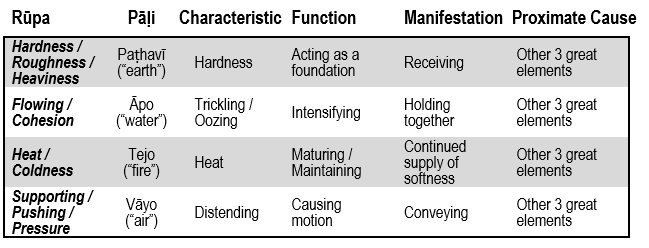
\includegraphics[width=0.8\linewidth]{./Diagrams/Elements}
\caption{The Four Great Elements.}
\label{fig:Elements}
\end{figure}

In the Suttas, the Buddha defined \textit{rūpas} as consisting of the Four Great Elements and \textit{rūpas} that depends on these elements.\footnote{MN 28: \url{http://www.accesstoinsight.org/tipitaka/mn/mn.028.than.html}} The Four Great Elements are \textbf{Earth-element}, \textbf{Water-element}, \textbf{Fire-element} and \textbf{Air-element}. Nowhere in the Suttas does the Buddha list the \textit{rūpas} that depend on the Four Great Elements. The \textit{rūpas} that depend on the Four Great Elements are defined in the Abhidhamma and in the Commentaries.

The word “element” tells us to focus on the properties rather than on the literal meaning of earth, water, fire or air. The Four Great Elements are experiences, Ultimate Realities, not concepts. The ancient Greeks and others\footnote{\url{http://en.wikipedia.org/wiki/Classical_element}} used the same four elements to describe the composition of the world, but generally adopted the literal or symbolic meaning rather than the Buddhist approach that focuses on properties. \textit{Rūpas} are not abstract categories; they are the realities that appear in daily life.

\textbf{Earth-element} is the experience of hardness or softness, roughness or smoothness, heaviness or lightness. Here are some exercises to experience \textbf{Earth-element}. Be aware of hardness in the teeth; bite them together and feel how hard they are. Be aware of softness by pressing your tongue against the inside of your lips to feel its softness. Rub your tongue over the edge of your teeth or brush your hand over the skin of your arm and feel roughness. Experience smoothness by wetting your lips and rubbing your tongue over them, from side to side. Place one hand on top of the other in your lap and feel the heaviness of the top hand, or feel the heaviness of the head by bending it forward. Look for lightness by wagging a finger up and down and feeling its lightness. If something floats in the ocean, it is because the \textbf{Earth-element} in the ocean supports it. If a balloon floats, it is because the \textbf{Earth-element} in the air supports it.

\textbf{Water-element} is flowing and cohesion. Flowing and cohesion cannot be experienced, but it can be understood by the mind. To understand flowing, imagine the blood flowing through the blood vessels, the air flowing into the lungs, or heat flowing throughout the body. To understand cohesion, consider how the body is held together by the skin, flesh, and sinews. The blood is held inside by the skin, like water in a balloon. Without cohesion the body would fall into separate pieces. The force of gravity which keeps the body stuck to the earth is also cohesion.

\textbf{Fire-element} is the experience of heat and coldness. It is usually very easy to look for heat throughout the body. Feel the coldness of the breath as it enters the nostrils and then understand it throughout the body. The function of \textbf{Fire-element} is to ripen, mature, age and burn up. The \textbf{Fire-element} also aids in digestion.

\textbf{Air-element} is the experience of supporting and pushing. To experience supporting, relax your back so your body bends forward. Then straighten it and keep it straight. The force that keeps the body straight is supporting. The supporting \textbf{Air-element} ensures that all things maintain their shape and do not collapse. To experience pushing, be aware through the sense of touch of pushing in the centre of the head as you breathe in and out, or experience the pushing as the chest expands or as the abdomen moves when breathing. Wherever there is movement, there is pushing. Though the function of \textbf{Air-element} is causing motion, movement is not the alteration between two stages of the same group of \textit{rūpas}, but rather the disappearance of one group of \textit{rūpas}, and the immediate emergence in its place of another group of \textit{rūpas}. For example, in a movie theatre, many static frames are projected onto the screen each second and a sense of movement is created.

All groups of \textit{rūpas} include the Four Great Elements. In a stone and a snowflake, the Four Great Elements exist in equal proportion, but of varying intensity. The intensity and the Mental Factor of \textbf{Attention} determine which experience body-consciousness recognizes first. For example, when you put your hand in water, the softness felt is \textbf{Earth-element}, the coolness felt is \textbf{Fire-element} and the pressure felt is \textbf{Air-element}. If the water is cold, then the \textbf{Fire-element} may be experienced first. If there is attention being paid to the sensation of pressure, then \textbf{Air-element} may be experienced first.

\subsection*{Sense Objects\footnote{Explained in Chapter 4 of “The Buddhist Teaching on Physical Phenomena” (see footnote 2).}}

\begin{figure} [h]
\centering
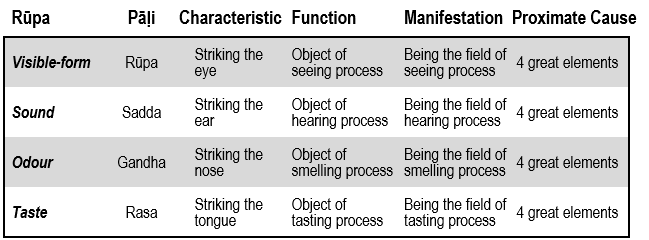
\includegraphics[width=0.8\linewidth]{./Diagrams/Objects}
\caption{The four sense objects (the sense objects of the tactile sense are \textbf{Hardness} (\textbf{Earth-element}), \textbf{Heat} (\textbf{Fire-element}) and \textbf{Supporting} (\textbf{Air-element}).}
\label{fig:Objects}
\end{figure}

\textbf{Earth-element}, \textbf{Fire-element} and \textbf{Air-element} are objects of the tactile sense, the sense of touch. The next set of \textit{rūpas} (\textbf{Visible-form},\footnote{Defined in Visuddhimagga XIV.54 (see footnote 2).} \textbf{Sound},\footnote{Defined in Visuddhimagga XIV.55 (see footnote 2).} \textbf{Odour}\footnote{Defined in Visuddhimagga XIV.56 (see footnote 2).} and \textbf{Taste}\footnote{Defined in Visuddhimagga XIV.57 (see footnote 2).}) are objects of the other four senses. The objects of the tactile sense are great elements; they have a strong impact and therefore, the accompanying \textbf{Feeling} of body-consciousness is either painful or pleasurable.\footnote{Thought Moment \textbf{17} is body-consciousness with painful \textbf{Feeling} and Thought Moment \textbf{24} is body-consciousness with pleasurable \textbf{Feeling}. Thought Moments \textbf{13}--\textbf{16} and \textbf{20}--\textbf{23} arise with indifferent \textbf{Feeling}.} The other sense objects have a weak impact, and therefore eye-consciousness, ear-consciousness, etc., are accompanied by indifferent \textbf{Feeling}.

Let’s look at \textbf{Visible-form} in a bit more detail. The Suttas and the Abhidhamma use the word \textit{rūpa} to mean both \textbf{Visible-form} and matter in general, so you must consider the context when you read the word “\textit{rūpa}.” \textbf{Visible-form} is colour; colour is what is actually seen by the eye.\footnote{The eye actually sees blue, green and red: \url{http://en.wikipedia.org/wiki/Photoreceptor_cell}} Once colour is seen by the eye, thinking takes place to create shapes and things. The eye does not see a cup; it sees colour, and the mind then creates a shape from colours; it creates things such as a cup. It can be difficult to know what \textbf{Visible-form} is because we are usually caught up in concepts such as a cup. The ear does not hear a song, the ear hears a single \textbf{Sound} and the mind uses many single \textbf{Sounds} to create a song.

In conventional language we might say, “I see my wife walking,” but the only Ultimate Reality in this example is a very small patch of colour somewhere in the field of vision.\footnote{Extend your arm and look at your thumbnail; this is the size of the portion of the field of vision that the retina can process at one time. The eye is constantly moving to build a complete visual image.} Everything else is added by the mind. As mentioned in the talk on Thought Moments, whenever something is added by the mind, there is an opportunity for latent fears and latent \textbf{Attachment} to distort and misinterpret. Modern research into eye movement\footnote{\url{http://en.wikipedia.org/wiki/Eye_movement}} has shown that the mind filters the visual scene by causing the eye to focus on areas of high contrast, to focus on faces or on movement. In other words, the mind naturally distorts and filters what is perceived.

The same principle applies to other senses; for example, consider the difference in hearing a language you understand and hearing a language you do not understand. When hearing a language you understand, the mind automatically creates words and ideas to accompany the sounds.

Imagine that you are sitting quietly in a meditation hall and somebody starts speaking outside. If the mind is interested in what is being said, the senses are not being guarded. If the mind is angry at the speaker, the senses are not being guarded. Getting caught up in a sense object, looking for reasons not to be mindful of what is happening in the present moment, is not wholesome. If there is awareness of \textbf{Sound}, but nothing more, this is a wholesome Thought Moment and the senses are being guarded. Similarly, treating the hardness of a diamond as being the same as the hardness of a pebble is guarding the senses and not getting caught up in the concept of money.

Each sense object is either intrinsically undesirable or intrinsically desirable.\footnote{According to the Commentary to the Abhidhamma (Sammohavinodanī 1, 10--11), an object’s intrinsic nature is according to “average” men such as accountants, government officials, land-owners and merchants. A masochist may enjoy pain, but pain is still intrinsically undesirable.} For example, the \textbf{Odour} of garbage is intrinsically undesirable while the \textbf{Odour} of coffee is intrinsically desirable. When the \textbf{Odour} of garbage enters the nostrils, this is a condition for Thought Moment \textbf{15} to arise; nose-consciousness that is a result of past unwholesome kamma. When the \textbf{Odour} of coffee enters the nostrils, it is a condition for Thought Moment \textbf{22} to arise; nose-consciousness that is a result of past wholesome kamma. Touching something that is very hot or very cold is a condition for Thought Moment \textbf{17} to arise; result of past unwholesome kamma. Touching something that is close to body temperature is a condition for Thought Moment \textbf{24} to arise; result of past wholesome kamma. This will be explored in more detail during the talk on processes.

\subsection*{Sense Organs\footnote{Explained in Chapter 3 of “The Buddhist Teaching on Physical Phenomena” (see footnote 2).}}

\begin{figure}[h]
\centering
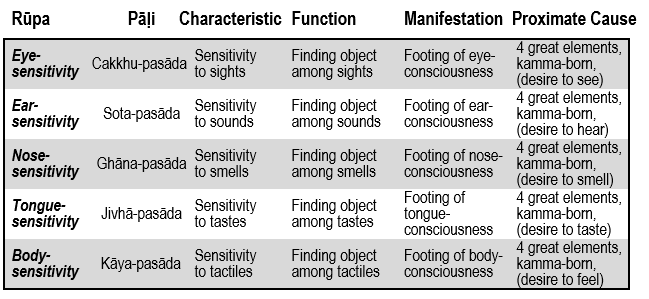
\includegraphics[width=0.8\linewidth]{./Diagrams/Organs}
\caption{The five sense organs.}
\label{fig:Organs}
\end{figure}

The next set of \textit{rūpas} are the sense organs. \textbf{Eye-sensitivity}\footnote{Defined in Visuddhimagga XIV.47 (see footnote 2).} is the portion of the eye that is capable of seeing colour; in other words, the retina. As mentioned in a previous talk, the Suttas explain that when \textbf{Visible-form} co-exists with the sensitive part of the eye, then eye-consciousness arises naturally. This does not mean that eye-consciousness is created by \textbf{Visible-form} striking the sensitive part of the eye;\footnote{\textbf{Visible-form} is external, so it cannot physically strike the sensitive part of the eye.} it means that \textbf{Visible-form} and a working sensitive part of the eye are necessary conditions for eye-consciousness to arise.

Just as \textbf{Eye-sensitivity} is located in the eye, \textbf{Ear-sensitivity}\footnote{Defined in Visuddhimagga XIV.49 (see footnote 2).} is located in the ear, \textbf{Nose-sensitivity}\footnote{Defined in Visuddhimagga XIV.50 (see footnote 2).} is located in the nose, \textbf{Tongue-sensitivity}\footnote{Defined in Visuddhimagga XIV.51 (see footnote 2).} is located on the tongue, and \textbf{Body-sensitivity}\footnote{Defined in Visuddhimagga XIV.52 (see footnote 2).} is located all over the body except for the hair, teeth and nails. \textbf{Body-sensitivity} is located wherever there are nerves to detect \textbf{Earth-element} such as hardness, \textbf{Fire-element} such as temperature and \textbf{Air-element} such as pressure.

The Abhidhamma also refers to the sense organs as doors. For example, \textbf{Eye-sensitivity} is the door through which the eye-consciousness Thought Moment reaches the \textbf{Visible-form}. Seeing happens at the eye-door, hearing happens at the ear-door, and so on. The Abhidhamma extends this analogy and refers to thinking as happening at the mind-door. So there are a total of six doors; five doors for the physical senses and the mind-door.

The Abhidhamma also refers to the sense organs as bases. A base supports the associated consciousness and is the location where the associated consciousness arises. The two types of eye-consciousness, Thought Moment \textbf{13} and Thought Moment \textbf{20}, arise at the eye-base, the retina. Similarly, the two types of ear-consciousness arise at the ear-base, the two types of nose-consciousness arise at the nose-base, the two types of tongue-consciousness arise at the tongue base and the two types of body-consciousness arise at the body-base.

Now we know where 10 of these Thought Moments, the two sets of fivefold sense consciousness, arise. But what about the remaining 79 Thought Moments that are listed in Handout 2? The Abhidhamma mentions that these Thought Moments arise based on “that \textit{rūpa} upon which the mind depends,” and the Commentary calls it the “\textbf{Heart-base}.” Just as eye-base supports eye-consciousness, ear-base supports ear-consciousness and so on, the \textbf{Heart-base} supports all the Thought Moments except for the 10 sense-consciousness.

\subsection*{Heart-base\footnote{Defined in Visuddhimagga XIV.60, explained in Chapter 5 of “The Buddhist Teaching on Physical Phenomena” (see footnote 2).}}

\begin{figure}[h]
\centering

\includegraphics[width=0.8\linewidth]{./Diagrams/Heart}
\caption{The \textbf{Heart-base} rūpa.}
\label{fig:Heart}
\end{figure}

According to the Abhidhamma, Thought Moments start to arise in a new existence immediately after conception. At that time, there is no heart (and no brain) to support these Thought Moments. This is why the Abhidhamma does not specify an organ as the base for the mind but rather uses the description, “that \textit{rūpa} upon which the mind depends.” \footnote{The term “Heart-base” is from the Commentary. The \textit{Dhammasaṅgaṇī} omits “Heart-base” from the list of \textit{rūpas} and the reference to “that \textit{rūpa} upon which the mind depends” is from the \textit{Paṭṭhāna}.}

In ancient times, people recognized that information sensed by different parts of the body needed to be collected in the mind. The only thing that was seen moving around the body was blood and the heart plays an obvious role in pumping blood. This is the basis of the view that the heart is the base for the mind that continues today in common speech. For example, you don’t say, “I love you with all my brain!” Interestingly, there are cases of heart transplant recipients “inheriting” characteristics from the donor.\footnote{\url{http://www.namahjournal.com/doc/Actual/Memory-transference-in-organ-transplant-recipients-vol-19-iss-1.html}}

\subsection*{Nutriment\footnote{Defined in Visuddhimagga XIV.70, explained in Chapter 2 of “The Buddhist Teaching on Physical Phenomena” (see footnote 2). }}

\begin{figure}[h]
\centering
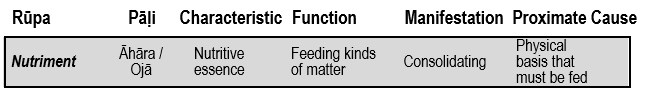
\includegraphics[width=0.8\linewidth]{./Diagrams/Nutriment}
\caption{The \textbf{Nutriment} rūpa.}
\label{fig:Nutriment}
\end{figure}

All groups of \textit{rūpas} include \textbf{Nutriment}; what we call “food” has a greater intensity of \textbf{Nutriment} \textit{rūpa}. \textbf{Nutriment} \textit{rūpa} can be ingested into the stomach or can come through external application such as eye drops or skin cream. According to the Suttas,\footnote{SN 12.63: \url{http://www.accesstoinsight.org/tipitaka/sn/sn12/sn12.063.than.html}} just as the body depends on the \textbf{Nutriment} \textit{rūpa}, the mind depends on the nutriment of \textbf{Contact}, \textbf{Volition} and consciousness.\footnote{In MN 9 (\url{http://www.accesstoinsight.org/tipitaka/mn/mn.009.than.html\#nutriments4}),\\ Sāriputta explains that properly discerning the four types of nutriment is Right View.}

\subsection*{Faculties\footnote{Explained in Chapter 5 of “The Buddhist Teaching on Physical Phenomena” (see footnote 2).}}

\begin{figure}[h]
\centering
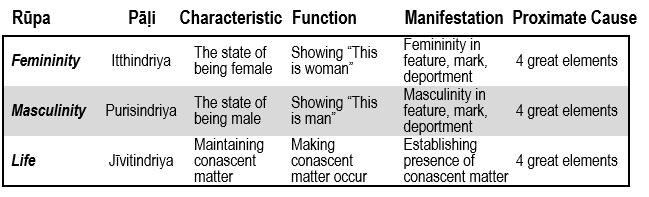
\includegraphics[width=0.8\linewidth]{./Diagrams/Faculties}
\caption{The three faculties.}
\label{fig:Faculties}
\end{figure}

\textbf{Life faculty},\footnote{Defined in Visuddhimagga XIV.59 (see footnote 2).} \textbf{Femininity-faculty} and \textbf{Masculinity-faculty}\footnote{Both defined in Visuddhimagga XIV.58 (see footnote 2).} are not localized; they are spread across the entire body just like the sense-organ of touch. Many women try to accentuate their \textbf{Femininity-faculty} and many men try to accentuate their \textbf{Masculinity-faculty}. This is \textbf{Attachment}; a desire to look feminine or to look masculine. Reminds me of a joke... women get married hoping that he will change and he doesn’t, men get married hoping that she will not change and he does. Tendencies tend to stay and the body always changes. Not getting what you want is dukkha\footnote{According to SN 6.63 (\url{http://www.accesstoinsight.org/tipitaka/an/an06/an06.063.than.html\#part-6}), “Birth is stress, ageing is stress, death is stress; sorrow, lamentation, pain, distress, \& despair are stress; association with the unloved is stress; separation from the loved is stress; not getting what is wanted is stress. In short, the five clinging-aggregates are stress.”}. When I was first married, I told my wife that I found her long hair to be very attractive. Twenty-five years later, my heart was filled with joy when she shaved her head to temporarily ordain as a Sayalay.

\subsection*{Material-\textit{rūpas} and Nominal-\textit{rūpas}}

The \textit{rūpas} listed above the thick line of Handout 5 are “material-\textit{rūpas};” they can be objects of \textit{vipassanā} meditation because they have the three characteristics of \textit{anicca}, \textit{dukkha} and \textit{anattā}. The \textit{rūpas} listed below the thick line of Handout 5 are “nominal-\textit{rūpas};” they are attributes or characteristics of the associated groups of material-\textit{rūpas} and are not valid objects of \textit{vipassanā} meditation.

\subsection*{Space\footnote{Defined in Visuddhimagga XIV.63, explained in Chapter 7 of “The Buddhist Teaching on Physical Phenomena” (see footnote 2).}}

\begin{figure}[h]
\centering
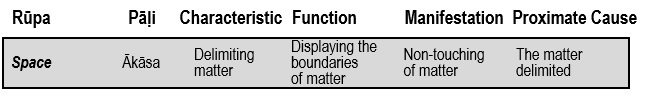
\includegraphics[width=0.8\linewidth]{./Diagrams/Space}
\caption{The \textbf{Space} rūpa.}
\label{fig:Space}
\end{figure}

The first nominal-\textit{rūpa} is space. Space does not exist as an Ultimate Reality, but some meditation teachers\footnote{For example, in the Pa-Auk method of meditation.} advise their students to concentrate on the space element to discern or infer the separation between different groups. Delimiting and separating groups allows the meditator to discern or infer the groups as being distinct. A rock is a cluster of many groups of \textit{rūpas}. Breaking up a rock shows there is space between the individual groups. A group of \textit{rūpas} is infinitesimally small, conceptually similar to an atom. However, one should not think of individual \textit{rūpa} as being like subatomic particles. For example, a group of \textit{rūpas} will have both \textbf{Hardness} and \textbf{Heat}; the \textbf{Hardness} and \textbf{Heat} cannot be separated but they can be sensed individually. As an analogy, a person has both height and weight; height and weight cannot be separated but they can be measured individually.

\subsection*{Indications\footnote{Explained in Chapter 6 of “The Buddhist Teaching on Physical Phenomena” (see footnote 2).}}

\begin{figure}[h]
\centering
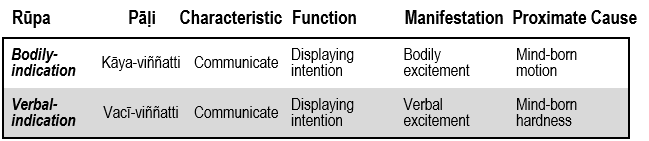
\includegraphics[width=0.8\linewidth]{./Diagrams/Indications}
\caption{The two indications.}
\label{fig:Indications}
\end{figure}

The next two nominal-\textit{rūpas} are the indications; \textbf{Bodily-indication}\footnote{Defined in Visuddhimagga XIV.61 (see footnote 2).} and \textbf{Verbal-indication}.\footnote{Defined in Visuddhimagga XIV.62 (see footnote 2).} These are intentional means of self-expression that may communicate one’s thoughts to another person or even to an animal.

Bodily movement involves a predominance of the mind-born \textbf{Air-element}, a material-\textit{rūpa}. When the \textbf{Air-element} of bodily movement is intentional, the group includes the nominal-\textit{rūpa} of \textbf{Bodily-indication}. \textbf{Bodily-indication} is an attribute of the bodily movement \textbf{Air-element}. If I nod my head as I doze off, this shows the mind-born \textbf{Air-element}. If I nod my head to indicate that I agree with you, the group also includes the nominal-\textit{rūpa} of \textbf{Bodily-indication}. \textbf{Bodily-indication} is not a material-\textit{rūpa}; it is a special attribute of the mind-born \textbf{Air-element} involved in bodily movement. \textbf{Bodily-indication} is not the gesture, it is the intentional aspect of a gesture that may communicate a message.

One’s voice arises from change of the mind-born \textbf{Earth-element} in the vocal cords. When the voice communicates a message, the group includes the nominal-\textit{rūpa} of \textbf{Verbal-indication}. \textbf{Verbal-indication} is an attribute of the mind-born \textbf{Earth-element} that is voice. If I use my voice to communicate a message to you, the group includes the nominal-\textit{rūpa} of \textbf{Verbal-indication}. \textbf{Verbal-indication} is not a material-\textit{rūpa}; it is a special attribute of the mind-born \textbf{Earth-element} involved in speaking. \textbf{Verbal-indication} is not the \textbf{Sound}, it is the intentional aspect of making a \textbf{Sound} that communicates a message.

\textbf{Bodily-indication} and \textbf{Verbal-indication} arise with intention as special attributes of mind-born material-\textit{rūpas}. If my stomach rumbles, there is no intention involved so this is not a mind-born group. A rumbling stomach is a temperature-born \textbf{Sound} group.

\subsection*{Agility, Pliancy and Adaptability\footnote{Defined in Visuddhimagga XIV.64, explained in Chapter 7 of “The Buddhist Teaching on Physical Phenomena” (see footnote 2).}}

\begin{figure}[h]
\centering
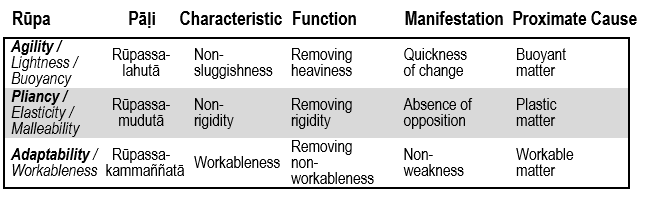
\includegraphics[width=0.8\linewidth]{./Diagrams/Agility}
\caption{\textbf{Agility} rūpa, \textbf{Pliancy} rūpa and \textbf{Adaptability} rūpa.}
\label{fig:Agility}
\end{figure}

The next three nominal-\textit{rūpas} are \textbf{Agility}, \textbf{Pliancy} and \textbf{Adaptability}. These \textit{rūpas} arise in groups that are part of the body and are attributes of physical health. When they arise in a temperature-born group, the body is healthy because of suitable climate. When they arise in a mind-born group, the body is healthy because of faultless Thought Moments. When they arise in a nutriment-born group, the body is healthy because of nutritious food. \textbf{Agility}, \textbf{Pliancy} and \textbf{Adaptability} are not distinct material-\textit{rūpas}; they are a sign that the body’s biological systems are in balance and healthy.

Buddhism emphasizes the importance of both mental health and physical health. Sometimes we need a reminder as to how important the mind is for the health of the body. In one Sutta, the Buddha visited a monk who was very ill.\footnote{SN 46.14: \url{http://www.accesstoinsight.org/tipitaka/sn/sn46/sn46.014.than.html}} The Buddha gave a short Dhamma talk and by reflecting on the Dhamma, the monk recovered from his sickness. The effect of the mind on the health of the body is well known to doctors. Mental stress leads to many health problems. A placebo will often improve a patient’s medical condition. We all know somebody whose positive attitude helped them through an illness. We should not wait until we are sick; wholesome Thought Moments will improve our health each moment and as it says in the Dhammapada, “Health is the greatest gift.” \footnote{See \url{http://www.tipitaka.net/tipitaka/dhp/verseload.php?verse=204}; in the Commentary to this verse, the Buddha advises King Pasenadi that it is not healthy to overeat.}

\textbf{Agility}, \textbf{Pliancy} and \textbf{Adaptability} are also names of Mental Factors that make wholesome Thought Moments non-sluggish, non-rigid and non-judgemental. The \textit{rūpas} of \textbf{Agility}, \textbf{Pliancy} and \textbf{Adaptability} imply a material-\textit{rūpa} that is healthy. When the body is not healthy, it is sluggish, rigid and not workable; it lacks the \textit{rūpas} of \textbf{Agility}, \textbf{Pliancy} and \textbf{Adaptability}.

\subsection*{Characteristics\footnote{Explained in Chapter 8 of “The Buddhist Teaching on Physical Phenomena” (see footnote 2).}}

\begin{figure}[h]
\centering
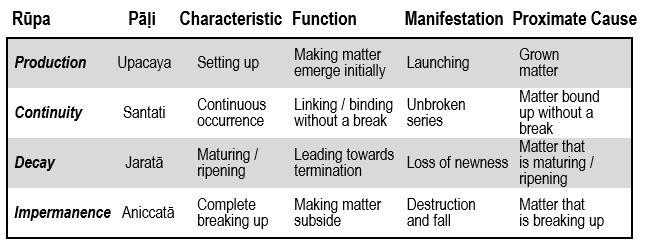
\includegraphics[width=0.8\linewidth]{./Diagrams/Characteristics}
\caption{The four characteristics.}
\label{fig:Characteristics}
\end{figure}

The final four nominal-\textit{rūpas} are \textbf{Production},\footnote{Defined in Visuddhimagga XIV.67 (see footnote 2).} \textbf{Continuity},\footnote{Defined in Visuddhimagga XIV.67 (see footnote 2).} \textbf{Decay},\footnote{Defined in Visuddhimagga XIV.68 (see footnote 2).} and \textbf{Impermanence}.\footnote{Defined in Visuddhimagga XIV.69 (see footnote 2).} These four \textit{rūpas} apply only to the body. Production starts from the moment of conception and continues until a complete set of \textit{rūpas} are created (the sense organs arise some time after conception). Continuity takes over once a complete set of \textit{rūpas} are created, and continuously refreshes the body throughout its lifespan. Decay is the inevitable ageing process such as grey hair and wrinkles that affect the body, and impermanence is the death of the body.

\subsection*{Groups of \textit{Rūpas}\footnote{Explained in Chapter 9 of “The Buddhist Teaching on Physical Phenomena” (see footnote 2).}}

We have finished describing the 28 \textit{rūpas}, so now let’s focus on how these \textit{rūpas} arise in groups.\footnote{In Pāḷi, these groups are called \textit{kalāpa}, a term that was introduced in the Commentaries.} As shown on the right side of Handout 5, there are four temperature-born groups, nine kamma-born groups (notice that the five sensitivities are shown in one column), six mind-born groups and two nutriment-born groups.

The body is made up of temperature-born groups, kamma-born groups, mind-born groups and nutrition-born groups. Things external to the body are made up of either temperature-born pure-octad groups or temperature-born \textbf{Sound} groups. A cup of coffee does not make a \textbf{Sound}, so it is made up of temperature-born pure-octad groups. A fan makes a \textbf{Sound}, so it is made up of temperature-born \textbf{Sound} groups.

From a Buddhist perspective, a cup of coffee and a fan are equivalent; they have the ability to be taken as sense objects. Plants do not have consciousness or kamma and are also made up of temperature-born pure-octad groups, unless they are making a \textbf{Sound}.

“Octad” means a collection of eight things; in this case, the eight \textit{rūpas} of \textbf{Earth-element}, \textbf{Water-element}, \textbf{Fire-element}, \textbf{Air-element}, \textbf{Visible-form}, \textbf{Odour}, \textbf{Taste} and \textbf{Nutriment}. All of the groups of \textit{rūpas} include these eight \textit{rūpas} as a foundation.\footnote{These are called “the eight inseparables” because they always arise as the foundation for every \textit{kalāpa}.}

\begin{figure}[h]
\centering
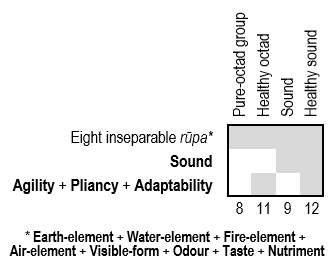
\includegraphics[width=0.5\linewidth]{./Diagrams/TempG}
\caption{A portion of Handout 5, reformatted to focus on the rūpas in the temperature-born groups.}
\label{fig:TempG}
\end{figure}

When the temperature-born pure-octad group is part of a healthy body, the \textit{rūpas} of \textbf{Agility}, \textbf{Pliancy} and \textbf{Adaptability} are present and this is the second group of \textit{rūpas}.

The temperature-born \textbf{Sound} group can be external to the body, such as a fan, or internal to the body such as a rumbling stomach. When the temperature-born \textbf{Sound} group is part of a healthy body, the \textit{rūpas} of \textbf{Agility}, \textbf{Pliancy} and \textbf{Adaptability} are present and this is the fourth group of \textit{rūpas}.

\textbf{Fire-element} arises in all groups of \textit{rūpas}. Irrespective of which group it arises in, \textbf{Fire-element} can be a condition for the arising of a new temperature-born group of \textit{rūpas}. A rock continues to be a rock, moment after moment, because temperature-born groups of \textit{rūpas} arise repeatedly.

\begin{figure}[h]
\centering

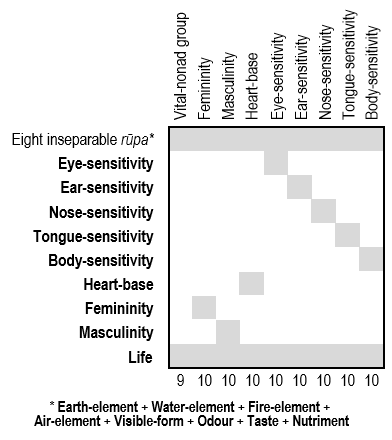
\includegraphics[width=0.5\linewidth]{./Diagrams/KammaG}
\caption{A portion of Handout 5, reformatted to focus on the rūpas in the kamma-born groups.}
\label{fig:KammaG}
\end{figure}

The next nine groups of \textit{rūpas} are kamma-born. These groups of \textit{rūpas} are part of the body. Life, gender, \textbf{Heart-base} and each of the five sense organs are the result of the same rebirth-linking kamma that gave rise to this existence. In Handout 5, the five types of sensitivities (\textbf{Eye-sensitivity}, \textbf{Ear-sensitivity}, etc.) have been compressed into a single column, but this one column represents five separate groups.

In the past existence there was \textbf{Attachment} to life, \textbf{Attachment} to femininity or masculinity and \textbf{Attachment} to sensing and thinking that led to this existence. An Arahat has uprooted all of these \textbf{Attachments} and therefore has no conditions for rebirth.

\begin{figure}[h]
\centering
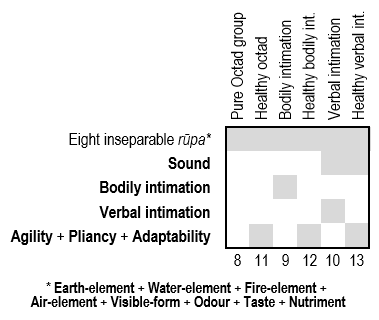
\includegraphics[width=0.5\linewidth]{./Diagrams/MindG}
\caption{A portion of Handout 5, reformatted to focus on the rūpas in the mind-born groups.}
\label{fig:MindG}
\end{figure}

\begin{figure}[h]
\centering
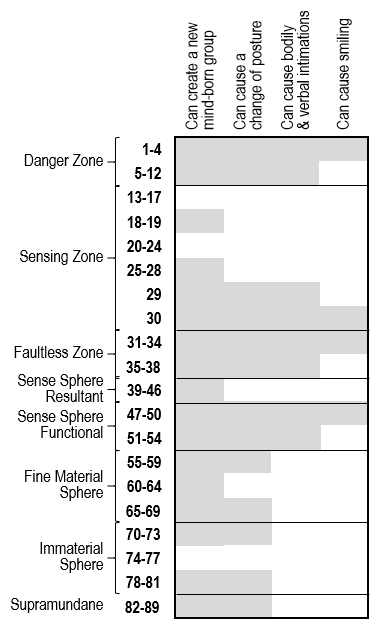
\includegraphics[width=0.5\linewidth]{./Diagrams/MindBorn}
\caption{Thought Moments (see Handout 2) and the mind-born groups that they can create.}
\label{fig:MindBorn}
\end{figure}

The next six groups of \textit{rūpas} are mind-born. These groups of \textit{rūpas} are part of the body. Almost all of the 89 Thought Moments create mind-born groups of \textit{rūpas}. The exceptions are the 10 sense-consciousness Thought Moments (they are too weak), and the four Life-continuum Thought Moments in the Immaterial Sphere. I will explain more about these Thought Moments in the next section when I talk about Realms of Existence.

\begin{figure}[h]
\centering

\includegraphics[width=0.5\linewidth]{./Diagrams/NutG}
\caption{A portion of Handout 5, reformatted to focus on the rūpas in the nutriment-born groups.}
\label{fig:NutG}
\end{figure}

The last two groups of \textit{rūpas} are nutriment-born. Nutriment-born groups of \textit{rūpas} are also part of the body. According to the Commentary, Nutriment \textit{rūpa} has the ability to produce new, nutriment-born groups of \textit{rūpas} for up to seven days after ingestion.

Most parts of the body include six groups of \textit{rūpas}: temperature-born pure-octad group (with or without health), kamma-born vital-nonad group, kamma-born gender (either femininity or masculinity) group, kamma-born Body-sensitivity group, mind-born pure-octad group (with or without health) and nutriment-born pure-octad group (with or without health). In other words, most parts of the body include three pure-octad groups (with or without health), vital-nonad group, either Femininity or Masculinity and Body-sensitivity. The physical eye includes seven groups of \textit{rūpas}; the same six groups of \textit{rūpas} as the rest of the body plus the kamma-born \textbf{Eye-sensitivity} group.

\subsection*{Linkage to \textit{Satipaṭṭhāna} Sutta}

Please refer to the \textit{Satipaṭṭhāna} Sutta printout. “The contemplation of the body” section, paragraphs 4 through 31 has many exercises dealing with \textit{rūpa}. Different meditation teachers tend to focus on different aspects of contemplation of the body, but most of them involve \textit{rūpa}. To conclude the section of the talk on \textit{rūpa}, I will give a couple of examples.

The most obvious example is paragraph 17, where the meditator is asked to consider the body as consisting of the four great elements. Focusing on the four great elements is an exercise in depersonalizing the body. The analogy in paragraph 18 of a butcher slaughtering a cow and dividing it into portions is explained in the Commentary as follows: when it is feeding in the pasture, being led to the slaughterhouse and when it is being killed, there is a perception of “cow.” When it is divided into portions, the perception of “cow” is replaced with a perception of “meat,” “blood” and “bones.” Considering the “cow” as its constituent parts depersonalizes the “cow.” \footnote{According to the Commentary, “the junction of four high roads” refers to the four postures of going, standing, sitting and lying down; in other words, at all times.}

As another example, in the Mahāsi Sayādaw approach to meditation, the mediator is asked to focus on the movement of the abdomen while breathing, and while walking, the meditator is asked to focus on the experiences of hardness, temperature and motion.

\subsection*{Summary of Key Points}

Here is a summary of key points regarding \textit{Rūpa}:

\begin{itemize}

\item \textit{Rūpas} includes all non-mental phenomena; a definition that is wider than the conventional translation of “matter.”

\item Buddhism focuses on spiritual development, so the Buddhist analysis of \textit{rūpa} focuses on sense objects, the sense organs and the body. 

\item The left side of Handout 5 is a glossary of the 28 \textit{rūpas}:

\begin{itemize}

\item Three of the “Four Great Elements” (\textbf{hardness} or \textbf{Earth-element}, \textbf{heat} or \textbf{Fire-element} and \textbf{supporting} or \textbf{Air-element}) are objects of the tactile sense. The fourth great element (\textbf{cohesion} or \textbf{Water-element}) is experienced by the mind.

\item The sense objects of \textbf{Visible-form}, \textbf{Sound}, \textbf{Odour} and \textbf{Taste} are the sense objects of the remaining senses.

\item The five sense organs (\textbf{Eye-sensitivity}, \textbf{Ear-sensitivity}, \textbf{Nose-sensitivity}, \textbf{Tongue-sensitivity} and \textbf{Body-sensitivity}) are able to detect sense objects (i.e. \textbf{Eye-sensitivity} is the portion of the retina that responds to light).

\item The \textbf{Heart-base} supports all Thought Moments except the sense-consciousness Thought Moments; these are supported by their respective sense organ (i.e. eye-consciousness Thought Moment arises at the retina).

\item \textbf{Nutriment} \textit{rūpa} includes food (though all groups of \textit{rūpas} include nutriment).

\item The three faculties (\textbf{femininity}, \textbf{masculinity} and \textbf{life}).

\item The remaining \textit{rūpas} are “nominal;” they are attributes of the associated group (“nominal” \textit{rūpas} are not valid objects of \textit{vipassanā}):

\begin{itemize}

\item \textbf{Space} separates the groups of \textit{rūpas}.

\item \textbf{Bodily-indication} and \textbf{verbal-indication} communicate information.

\item \textbf{Agility}, \textbf{pliancy} and \textbf{adaptability} are the attributes of physical health.

\item The four characteristics (\textbf{production}, \textbf{continuity}, \textbf{decay} and \textbf{impermanence}) represent the stages of life.

\end{itemize}

\end{itemize}

\item The right side of Handout 5 shows \textit{rūpas} included within each group:

\begin{itemize}

\item Non-living things are made up of \textbf{temperature-born pure-octad groups} or \textbf{temperature-born \textbf{Sound} groups}. Their relevance in the Buddhist analysis of \textit{rūpa} is that non-living things are merely sense objects.

\item Living things are made of all groups of \textit{rūpas} (four temperature-born groups, nine kamma-born groups, six mind-born groups and two nutriment-born groups).

\end{itemize}

\item The \textbf{\textit{R}} \textbf{\textit{A}} \textbf{\textit{D}} \textbf{\textit{I}} \textbf{\textit{CA}} \textbf{\textit{L}} process (\textbf{\textit{R}}ecognize, \textbf{\textit{A}}ccept, \textbf{\textit{D}}epersonalize, \textbf{\textit{I}}nvestigate, \textbf{\textit{C}}ontemplate \textbf{\textit{A}}\textit{nicca}/\textbf{\textit{C}}ontemplate \textbf{\textit{A}}\textit{nattā}, \textbf{\textit{L}}et go) can also be applied to \textit{rūpa} (except for “nominal” \textit{rūpas}).

\end{itemize}

Finally, in my opinion, the most important thing to remember about \textit{rūpa} is that, in the context of spiritual development, its main relevance is as a sense object. We don’t touch a pebble; hardness, temperature and pressure are experienced. “Pebble” is a concept. We don’t see a car. \textbf{Visible-form} is a small patch of colour experienced by the eye. “Car” is a concept. Guarding the senses means not getting caught up in concepts.

\begin{center}
\textbf{\textit{This concludes the fifth talk.}} \\
\end{center}

\newpage

\subsection*{Questions \& Answers}

\question{According to Buddhism, what is the role of the brain?}

In most of the Suttas (including paragraph 15 of the \textit{Satipaṭṭhāna} Sutta), there is a list of 31 parts of the body used to contemplate the repulsiveness of the body. There are some Suttas (added at a much later date) that expand this list to 32 parts of the body by adding the brain to the end of the list.\footnote{Khp 3: \url{http://www.accesstoinsight.org/tipitaka/kn/khp/khp.1-9x.piya.html\#khp-3}} Visuddhimagga VIII.126 describes the brain as the marrow of the skull bone and gives it no special significance (nothing related to the mind). In fact, Visuddhimagga VIII.136 describes snot coming out of the nose as originating in the brain!\footnote{I am glad that my doctor did not get his medical knowledge from the Visuddhimagga! \smiley} The Suttas and the Abhidhamma associate sense-consciousness with the sense organs but do not associate the mind with any organ (see discussion on the \textbf{Heart-base} \textit{rūpa}).

In an article, “Is your brain really necessary?” \footnote{\url{http://www.rifters.com/real/articles/Science\_No-Brain.pdf}} Dr. John Lorber says, “There’s a young student at this university, who has an IQ of 126, has gained a first-class honours degree in mathematics, and is socially completely normal. And yet the boy has virtually no brain. When we did a brain scan on him, we saw that instead of the normal 4.5-centimeter thickness of brain tissue between the ventricles and the cortical surface, there was just a thin layer of mantle measuring a millimeter or so. His cranium is filled mainly with cerebrospinal fluid.” In my opinion, there are still many gaps in our scientific knowledge regarding the relationship between mind and body.

\question{The Suttas\footnote{SN 22.48: \url{http://www.accesstoinsight.org/tipitaka/sn/sn22/sn22.048.than.html}} describe \textit{rūpas} as “past, future, or present; internal or external; blatant or subtle; common or sublime.” What does this mean?}

I believe that the intention of the Buddha was to indicate that all \textit{rūpas}, no matter how it might be subdivided or analyzed, is to be included. The Commentary to the Abhidhamma analyzes \textit{rūpa} according to these categories, but I treat this part of the Commentary as more of a scholarly exercise rather than being helpful, practical or useful.

\question{You mentioned that gender is determined by kamma. Is being reborn as a female the result of past unwholesome kamma?}

Nowhere in the Vinaya, in the Suttas or in the Abhidhamma does it imply that rebirth as a female is the result of past unwholesome kamma (though there are some stories in the Commentaries that reflect this sexist attitude).\footnote{For example, \url{http://www.tipitaka.net/tipitaka/dhp/verseload.php?verse=043}} Women were able to become Arahats, making them the spiritual equal of men. One of the books of the \textit{Tipiṭaka} is dedicated to verses written by nuns.\footnote{\url{http://en.wikipedia.org/wiki/Therigatha}} The Buddha did say that a Buddha cannot be a woman\footnote{MN 115: \url{http://awake.kiev.ua/dhamma/tipitaka/2Sutta-Pitaka/2Majjhima-Nikaya/Majjhima3/115-bahudhatuka-e.html}} (of course, a woman in this life could be reborn as a man in a future life and become a Buddha in that life). When King Pasenadi was displeased at having a daughter, the Buddha said, “A woman may turn out better than a man.” \footnote{SN 3.16 (The on-line translation is a bit convoluted, so I am using Bhikkhu Bodhi’s translation): \url{http://metta.lk/tipitaka/2Sutta-Pitaka/3Samyutta-Nikaya/Samyutta1/03-Kosala-Samyutta/02-Aputtakavaggo-e.html}}

Some monks object to the ordination of Theravāda Bhikkhunī. Their objection is not based on any perceived inferiority of females; it is based on their interpretation of what is allowable under the Vinaya. I have found the following website to be an excellent source of information: \url{http://sites.google.com/site/santipada/bhikkhunifaq} Another source of information is an article, “The Legality of Bhikkhunī Ordination” by Ven. Anālayo: \url{http://www.buddhismuskunde.uni-hamburg.de/pdf/5-personen/analayo/legality.pdf} I am a strong supporter of Theravāda Bhikkhunī ordination. 

Actually, the suggestion to prepare this Practical Abhidhamma Course came in 2014 from Ayyā Medhānandī Bhikkhunī, after a talk I gave at Sati Sārāņīya Hermitage (\url{http://satisaraniya.ca/}) in Ontario, Canada. I am \textbf{extremely} grateful to Ayyā Medhānandī.